% Modified Template by Jonathan Doucette and Kevin Multani, original by: Jonathan Ward

\documentclass[12pt]{article} 
\usepackage[english]{babel}
\usepackage[utf8]{inputenc}
\usepackage{amsmath} % AMS Math Package
\usepackage{amsthm} % Theorem Formatting
\usepackage{amssymb} % Math symbols such as \mathbb
\usepackage{graphicx} % Allows for eps images
\usepackage{multicol} % Allows for multiple columns
\usepackage[dvips,letterpaper,margin=1in,bottom=1in]{geometry}
\usepackage{hyperref}
\usepackage{parskip} % Removes indentation from paragraphs
\usepackage{xcolor,xspace,soul} % Colour, spacing, and highlighting
\usepackage{mathrsfs}
\usepackage{bm} % For bold math symbols
\usepackage{amscd}
\usepackage[all,cmtip]{xy}
%\usepackage{bbm}
\usepackage{titling}
\usepackage{listing} % for code snippets
%\usepackage{minted} % for code snippets
\usepackage{enumerate}
\usepackage{fancyhdr}
\usepackage[]{physics}
\usepackage[makeroom]{cancel}
\usepackage{pdfpages}
\usepackage[]{mcode}
\usepackage[title]{appendix}

% ***********************************************************
% ********************** BEGIN TITLE PAGE *******************
% ***********************************************************
\newcommand*{\titleGM}{\begingroup % Create the command for including the title page in the document
\hbox{ % Horizontal box
\hspace*{0.2\textwidth} % Whitespace to the left of the title page
\rule{1pt}{\textheight} % Vertical line
\hspace*{0.05\textwidth} % Whitespace between the vertical line and title page text
\parbox[b]{0.75\textwidth}{ % Paragraph box which restricts text to less than the width of the page

{\noindent\Huge\bfseries MATH 521}\\[2\baselineskip] % Title
{\large \textit{Assignment 4}}\\[4\baselineskip]
%{\large \textsc{ Jonathan Doucette }} % Author name

\vspace{0.5\textheight} % Whitespace between the title block and the publisher
{\noindent \today }\\[\baselineskip]
%{\noindent Student Number: 35298124 }\\[\baselineskip] 
%{\noindent \footnotesize All problems below are \textit{Copyright \copyright \space 2018 Timm Treskatis. All Rights Reserved.} }\\[\baselineskip]
} % end parbox
} % end hbox
\endgroup}

 % Sets margins and page size
\pagestyle{fancy} 

%\lhead{Jonathan Doucette}
\rhead{\today}
\rfoot{Page \thepage}
\cfoot{}

\makeatletter % Need for anything that contains an @ command 
\renewcommand{\maketitle} % Redefine maketitle to conserve space
{ \begingroup \vskip 10pt \begin{center} \Huge {\bf \@title}
\vskip 10pt \large \@author \hskip 20pt \@date \end{center}
  \vskip 10pt \endgroup \setcounter{footnote}{0} }
\makeatother % End of region containing @ commands

% ***********************************************************
% ********************** END TITLE PAGE *********************
% ***********************************************************

% ***********************************************************
% ********************** BEGIN NEW COMMANDS *****************
% ***********************************************************

\renewcommand{\labelenumi}{(\alph{enumi})} % Use letters for enumerate
\let\vaccent=\v % rename builtin command \v{} to \vaccent{}

%% MISC
\newcommand{\ab}[1]{\left| #1 \right|} % for absolute value
\newcommand{\avg}[1]{\left< #1 \right>} % for average
\let\underdot=\d % rename builtin command \d{} to \underdot{}
\let\baraccent=\= % rename builtin command \= to \baraccent
\renewcommand{\=}[1]{\stackrel{#1}{=}} % for putting numbers above =
\providecommand{\fr}{\frac}
\providecommand{\RR}{\mathbb{R}}
\providecommand{\CC}{\mathbb{C}}
\providecommand{\NN}{\mathbb{N}}
\providecommand{\e}{\epsilon}
\DeclareMathOperator{\di}{d\!}
\newcommand*\ieval[3]{\left.#1\right\rvert_{#2}^{#3}}

%% Vectors
\renewcommand{\v}[1]{\ensuremath{\mathbf{#1}}} 
\newcommand{\gv}[1]{\ensuremath{\mbox{\boldmath$ #1 $}}} % for vectors of Greek letters
\newcommand{\uv}[1]{\ensuremath{\mathbf{\hat{#1}}}} % for unit vector
\providecommand{\wave}[1]{\v{\tilde{#1}}}

%% DERIVATIVES
\renewcommand{\d}[2]{\frac{d #1}{d #2}} % for derivatives
\newcommand{\dubd}[2]{\frac{d^2 #1}{d #2^2}} % for double derivatives
\newcommand{\pd}[2]{\frac{\partial #1}{\partial #2}} % for partial derivatives
\newcommand{\pdd}[2]{\frac{\partial^2 #1}{\partial #2^2}} % for double partial derivatives

%% Operators
\newcommand{\Gradient}{\ensuremath{\mbox{\boldmath$\nabla$}}} % gradient

%% Text
\newcommand{\mathcolorbox}[2]{\colorbox{#1}{$\displaystyle #2$}}
\newcommand{\hlfancy}[3]{\textcolor{#1}{\sethlcolor{#2}\hl{#3}}}
\newcommand{\TODO}[1]{\hlfancy{red}{yellow}{\textbf{TODO: #1}}}

%% Code
%\newcommand{\code}[1]{\mintinline{C}{#1}}
%\newcommand{\code}[1]{\texttt{#1}}
\newcommand{\code}[1]{\lstinline[columns=fixed]{#1}}
\newcommand{\includecode}[1]{\lstinputlisting{#1}}

% ***********************************************************
% ********************** END NEW COMMANDS *******************
% ***********************************************************

% ***********************************************************
% ********************** BEGIN NEW ENVS *********************
% ***********************************************************

% Theorem
\newenvironment{theorem}[2][Theorem]{\begin{trivlist}
\item[\hskip \labelsep {\bfseries #1}\hskip \labelsep {\bfseries #2.}]}{\end{trivlist}}
% Lemma
\newenvironment{lemma}[2][Lemma]{\begin{trivlist}
\item[\hskip \labelsep {\bfseries #1}\hskip \labelsep {\bfseries #2.}]}{\end{trivlist}}
% Corollary
\newenvironment{corollary}[2][Corollary]{\begin{trivlist}
\item[\hskip \labelsep {\bfseries #1}\hskip \labelsep {\bfseries #2.}]}{\end{trivlist}}

% Exercise
\newenvironment{exercise}[2][Exercise]{\begin{trivlist}
\item[\hskip \labelsep {\bfseries #1}\hskip \labelsep {\bfseries #2.}]}{\end{trivlist}}
% Problem
\newenvironment{problem}[2][Problem]{\begin{trivlist}
\item[\hskip \labelsep {\bfseries #1}\hskip \labelsep {\bfseries #2.}]}{\end{trivlist}}
% Question
\newenvironment{question}[2][Question]{\begin{trivlist}
\item[\hskip \labelsep {\bfseries #1}\hskip \labelsep {\bfseries #2.}]}{\end{trivlist}}
% Solution
\newenvironment{solution}{\begin{proof}[Solution]}{\end{proof}}

% Afterword
\newenvironment{afterword}[2][Appendix]{\begin{trivlist}
\item[\hskip \labelsep {\bfseries #1}\hskip \labelsep {\bfseries #2}]}{\end{trivlist}}

% ***********************************************************
% ********************** END NEW ENVS ***********************
% ***********************************************************

% ***********************************************************
% ********************** END TITLEPAGE **********************
% ***********************************************************

\begin{document}

\begin{frame}
\titlepage
\begin{textblock*}{2cm}(1.3cm,-3.3cm)
    
\includegraphics[height=2cm]{figures/ubc-logo}
\end{textblock*}
\begin{textblock*}{2cm}(9cm,-3.3cm)
    
\includegraphics[height=2cm]{figures/UBC-MRI-logo}
\end{textblock*}
\end{frame}

%\begin{frame}
%\tableofcontents
%%TODO
%\TODO{uncomment all ``pause'' statements}
%\end{frame}


\section{Background}

\subsection{Magnetic Resonance Visualised}

% Visualisation of the bulk magnetization. Initially, all magnetised spins are aligned with the main magnetic field. 90 deg RF pulse kicks them into the xy-plane, and they begin to dephase. Note: this is RELATIVE spin rates; all spins are rotating in nearly the same direction, in fact, the relative rate between them differs by only ~1 part in 10^6
\begin{frame}
\frametitle{Magnetic Resonance Visualised}
\begin{enumerate}
    \item Animation of a typical ``spin echo'' MRI sequence
    %\item \TODO{re-compile with animated gif} %TODO
\end{enumerate}
\centering
\animategraphics[loop,controls,width=0.7\linewidth]{25}{gifs/HahnEcho_GWM-}{0}{255}
%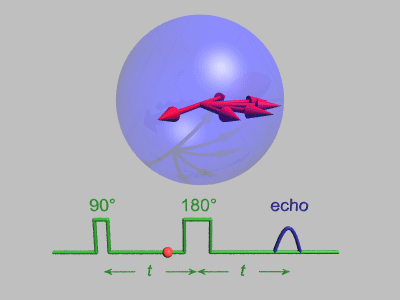
\includegraphics[width=0.7\linewidth]{gifs/HahnEcho_GWM-100}
\end{frame}

\begin{frame}
\frametitle{Magnetic Resonance Visualised}
%\begin{enumerate}
%    \item In actuality, spins (water molecules) do not truly fully refocus
%    %\pause
%    \item Relative angular frequency depends on local magnetic field, and therefore spins dephase at different rates at different locations
%    %\pause
%    \item In particular, the \textbf{diffusion} of spins during the scan ($\approx$ \SI{40}{\milli\second}) leads to a net lost in signal: \underline{the ``echo'' is weaker}
%\end{enumerate}
\begin{enumerate}
    \item Spins (water molecules) do not truly refocus:
    \pause
    \begin{enumerate}
        \item Precession rate depends on position
        \pause
        \item Diffusion plays an important role
    \end{enumerate}
\end{enumerate}
\centering
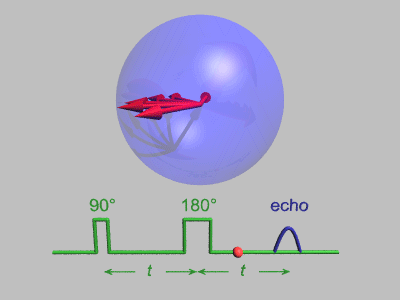
\includegraphics[width=0.55\linewidth]{gifs/HahnEcho_GWM-165}
\end{frame}

\begin{frame}
\frametitle{Magnetic Resonance Visualised}
\centering
%\vspace{-0.5cm}
\begin{columns}
\begin{column}{.5\textwidth}
\begin{figure}
  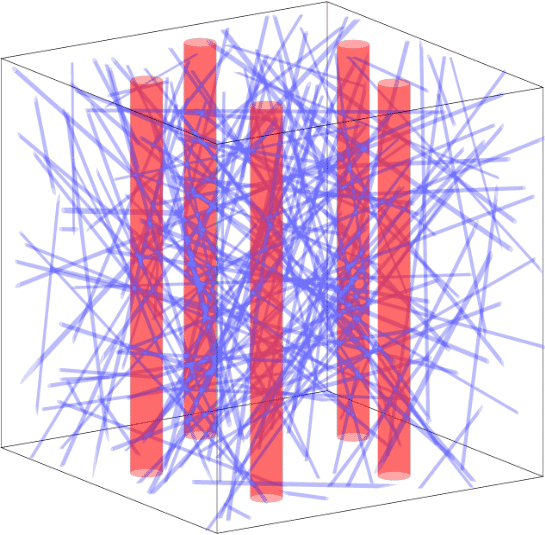
\includegraphics[height=0.8\textwidth]{figures/voxelgeo}
  \caption{Simulated imaging voxel}
%  \caption{Cubic imaging voxel filled with randomly oriented microvasculature}
\end{figure}
\end{column}
%\hfill
\begin{column}{.5\textwidth}
\begin{figure}
  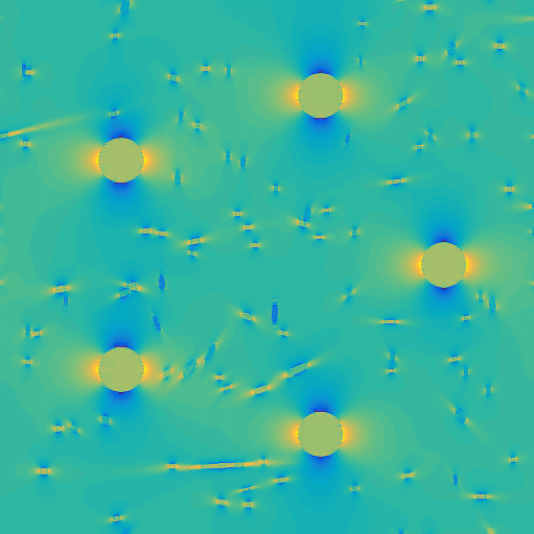
\includegraphics[height=0.8\textwidth]{figures/domega}
  \caption{Cross section of precession rate}
%  \caption{Cross section of $\omega$ corresponding to the microvasculature filled voxel}
\end{figure}
\end{column}
\end{columns}
\end{frame}

\subsection{The Bloch-Torrey Equation}

\begin{frame}
\frametitle{The Bloch-Torrey Equation}
\begin{enumerate}
    \item Evolution of the magnetization is modelled by the \textbf{Bloch-Torrey equation}
    $$ \pd{\Mxy}{t} = D \Laplacian{\Mxy} - \CDecay \Mxy $$
    where:
    \begin{align*}
        \Mxy &= M_x + i \, M_y \\
        \CDecay(\v{x}) &= R(\v{x}) + i \, \omega(\v{x})
    \end{align*}
    \pause
    \item IC: $\Mxy(\v{x},0) = \Mxy_0(\v{x})$ is given
    \pause    
    \item BC: zero Neumann or periodic
    \pause
    \item Note:
    $$ D = 0 \, \Rightarrow \, \Mxy(\v{x},t) = \Mxy_0(\v{x}) e^{-\CDecay(\v{x}) t} $$
\end{enumerate}
\end{frame}

\section{Solving the Bloch-Torrey Equation}


\subsection{Operator Splitting Methods}

\begin{frame}
\frametitle{Operator Splitting Methods}
\begin{enumerate}
    %\item One effective method of solving the BT equation is via \textit{operator splitting methods}
    %\pause
    \item First, the BT PDE is rewritten in the more suggestive form
    $$ \pd{\Mxy}{t} = H \Mxy $$
    where
    \begin{gather*}
        H = -D \Laplacian{} + \CDecay.
    \end{gather*}
    \pause
    \item Then, the general solution $\Mxy$ may then be written as
    $$ \Mxy = e^{-Ht}\Mxy_0 $$
    where $e^{-Ht}$ is the \textit{evolution operator}
\end{enumerate}
\end{frame}

\begin{frame}
\frametitle{Operator Splitting Methods}
\begin{enumerate}
    \item Now, the evolution operator may be \textit{split} using the approximation %TODO ref
    \begin{align*}
        e^{-Ht} &= e^{D \Delta t - \CDecay t} \\
        &\approx e^{-\CDecay t/2} e^{D \Delta t} e^{-\CDecay t/2} + \mathcal{O}(t^3)
    \end{align*}
    %\pause
    %\item This form is advantageous because although $e^{-Ht}$ has no closed form for general $\CDecay$, the split operators do:
    \pause
    \item Although $e^{-Ht}$ has no closed form, the split operators do:
    \begin{align*}
        e^{-\Gamma t/2} \Mxy &= e^{-\Gamma(\v{x}) t/2} \odot \Mxy \\
        e^{D \Delta t} \Mxy &= \Phi \conv \Mxy
    \end{align*}
    %where $\odot$ is the Hadamard (pointwise) product, $\conv$ is the spatial convolution, and $\Phi$ is a Gaussian smoothing kernel with $\sigma = \sqrt{2Dt}$
\end{enumerate}
\end{frame}

\subsection{Finite Element Methods}

\begin{frame}
\frametitle{Finite Element Methods}
\begin{enumerate}
    \item The BT equation can also be solved using FEM
    \pause
    \item First, let $u=M_x$ and $v=M_y$ and write:% and rewrite the complex Bloch-Torrey PDE as a pair of coupled real PDE's:
    \begin{equation*}
    \begin{cases}
        \pd{u}{t} = D \Laplacian{u} - R u + \omega v\\%, \qquad u(\v{x},0) = M_x(\v{x},0) \\
        \hspace{0.5pt}\pd{v}{t} = D \Laplacian{v} - R v - \omega u\\%, \qquad \hspace{1pt} v(\v{x},0) = M_y(\v{x},0)
    \end{cases}
    \end{equation*}
%    with
%    \begin{align*}
%        u(\v{x},0) &= M_x(\v{x},0) \\
%        v(\v{x},0) &= M_y(\v{x},0)
%    \end{align*}
%    %\pause
%    \item Writing the pair of PDE's as a linear system results in
%    \begin{align*}
%    \pd{}{t}
%    \begin{pmatrix} u \\ v \end{pmatrix}
%    = \begin{pmatrix}
%    D \Laplacian{} - R & \omega \\ 
%    -\omega & D \Laplacian{} - R
%    \end{pmatrix}
%    \begin{pmatrix} u \\ v \end{pmatrix}
%    \end{align*}
\end{enumerate}
\end{frame}

%\begin{frame}
%\frametitle{Finite Element Methods}
%\vspace{-0.5cm}
%\begin{align*}
%    \pd{}{t}
%    \begin{pmatrix} u \\ v \end{pmatrix}
%    = \begin{pmatrix}
%    D \Laplacian{} - R & \omega \\ 
%    -\omega & D \Laplacian{} - R
%    \end{pmatrix}
%    \begin{pmatrix} u \\ v \end{pmatrix}
%\end{align*}
%\vspace{-0.25cm}
%\begin{enumerate}
%    \item If we take the inner product of both sides with $\begin{pmatrix} u \;\, v \end{pmatrix}^T$, we have that
%    \begin{align*}
%    \int_\Omega u u_t + v v_t \dx{x}
%    &= \int_\Omega D u \Laplacian{u} - R u^2 + D v \Laplacian{v} - R v^2 \dx{x} \\
%    &= \int_\Omega -D \, (||\nabla u||^2 + ||\nabla v||^2) - R \, (u^2 + v^2) \dx{x} \\
%    &< 0 \quad \text{for u,v} \, \not\equiv 0
%    \end{align*}
%    \item Now, $ \int_\Omega u u_t + v v_t \dx{x} = \frac{1}{2} \pd{}{t} \left( \int_\Omega u^2 + v^2 \dx{x} \right) = \frac{1}{2} \pd{}{t} \LTwoNorm{\Mxy}^2$, and so
%    $$ \pd{}{t} \LTwoNorm{\Mxy(\v{x},t)} < 0 $$
%    Therefore, the magnitude of the transverse magnetization decreases with time
%    %\item Additionally, it is clear that the presence of diffusion increases the rate of decrease
%\end{enumerate}
%\end{frame}

\begin{frame}
\frametitle{Finite Element Methods}
\begin{enumerate}
    \item Applying the method of lines:%, the pair of PDE's becomes
    \begin{align*}
        M^h \v{u}_t &= -(D K^h + R^h) \v{u} + W^h \v{v} \\
        M^h \v{v}_t &= -(D K^h + R^h) \v{v} - W^h \v{u}
    \end{align*}
    where:% $R^h_{ij} \coloneqq \int R \,\phi_i \,\phi_j \dx{x}$, $W^h_{ij} \coloneqq \int \omega \,\phi_i \,\phi_j \dx{x}$, and $M^h$ and $K^h$ are the usual mass and stiffness matrices
    \begin{align*}
        R^h_{ij} &\coloneqq \int R \,\phi_i \,\phi_j \dx{x} \\
        W^h_{ij} &\coloneqq \int \omega \,\phi_i \,\phi_j \dx{x}
    \end{align*}
%    %\pause
%    \item $M^h$, $K^h$, and $R^h$ are symmetric positive definite; $W^h$ is symmetric
%    %\pause
%    \item In choosing a time 
%discretization, first consider the block system:
%    \begin{align*}
%    \begin{pmatrix}
%    M^h & 0 \\ 
%    0 & M^h
%    \end{pmatrix}
%    \pd{}{t}
%    \begin{pmatrix} \v{u} \\ \v{v} \end{pmatrix}
%    = -
%    \begin{pmatrix}
%    A^h & -W^h \\ 
%    W^h & A^h
%    \end{pmatrix}
%    \begin{pmatrix} \v{u} \\ \v{v} \end{pmatrix}
%    \end{align*}
%    \\ where $A^h \coloneqq D K^h + R^h$ is symmetric positive definite
\end{enumerate}
\end{frame}
\frametitle{Finite Element Methods}
%\vspace{-1cm}
%\begin{align*}
%    \begin{pmatrix}
%    M^h & 0 \\ 
%    0 & M^h
%    \end{pmatrix}
%    \pd{}{t}
%    \begin{pmatrix} \v{u} \\ \v{v} \end{pmatrix}
%    = -
%    \begin{pmatrix}
%    A^h & -W^h \\ 
%    W^h & A^h
%    \end{pmatrix}
%    \begin{pmatrix} \v{u} \\ \v{v} \end{pmatrix}
%\end{align*}
%\begin{enumerate}
%    \item If we take the inner product of both sides with $\begin{pmatrix} \v{u}^T, \v{v}^T \end{pmatrix}$, we have that
%    \begin{align*}
%    \pd{}{t}
%    \left( \v{u}^T M^h \v{u} + \v{v}^T M^h \v{v} \right)
%    %&= - \left( \v{u}^T A^h \v{u} - \v{u}^T W^h \v{v} + \v{v}^T W^h \v{u} + \v{v}^T A^h \v{v} \right) \\
%    &= - \left( \v{u}^T A^h \v{u} + \v{v}^T A^h \v{v} \right)
%    \quad \text{by symmetry of } W^h \\
%    &\leq 0 \quad \text{by positive definiteness of } A^h
%    \end{align*}
%    %\pause
%    \item Now, $\LTwoNorm{\bm{\Mxy}}^2 = \v{u}^T M^h \v{u} + \v{v}^T M^h \v{v}$, and so $\LTwoNorm{\bm{\Mxy}}$ decreases with time
%    %\pause
%    \item For this reason, the second order and strongly A-stable time stepping \textsc{TR-BDF2} was used
%\end{enumerate}
%\end{frame}

\subsection{Time Stepping}

\begin{frame}
\frametitle{Time Stepping Methods}
%\begin{align*}
%    \begin{pmatrix}
%    M^h & 0 \\ 
%    0 & M^h
%    \end{pmatrix}
%    \pd{}{t}
%    \begin{pmatrix} \v{u} \\ \v{v} \end{pmatrix}
%    = -
%    \begin{pmatrix}
%    A^h & -W^h \\ 
%    W^h & A^h
%    \end{pmatrix}
%    \begin{pmatrix} \v{u} \\ \v{v} \end{pmatrix}
%\end{align*}
\begin{align*}
        M^h \v{u}_t &= -(D K^h + R^h) \v{u} + W^h \v{v}\\
        M^h \v{v}_t &= -(D K^h + R^h) \v{v} - W^h \v{u}
\end{align*}
\vspace{-0.5cm}
\begin{enumerate}
    \item Solutions to the Bloch-Torrey equation decay exponentially in time and smooth high frequency modes
%    \begin{align*}
%        - \begin{pmatrix} \v{u}^T \, \v{v}^T \end{pmatrix}
%        \begin{pmatrix}
%        A^h & -W^h \\ 
%        W^h & A^h
%        \end{pmatrix}
%        \begin{pmatrix} \v{u} \\ \v{v} \end{pmatrix}
%        &= - \v{u}^T A^h \v{u} - \v{v}^T A^h \v{v} \\
%        &< 0 \quad \text{for \v{u},\v{v}} \, \neq \v{0}
%    \end{align*}
%    %\pause
%    \item The time 
%discretization scheme should therefore be at least strongly A-stable to reflect this
    \pause
    \item Strongly A-stable time stepping methods are required %and second order accurate time stepping scheme \textsc{TR-BDF2} was used
\end{enumerate}
\end{frame}


\section{Results}

\subsection{Operator Splitting versus FEM}

%\begin{frame}
%\frametitle{Operator Splitting versus FEM}
%\begin{enumerate}
%    \item Comparing the solution of the BT equation with splitting methods versus FEM...
%    \item \TODO{do this} %TODO
%\end{enumerate}
%\end{frame}

\begin{frame}
\frametitle{Operator Splitting versus FEM}
\centering
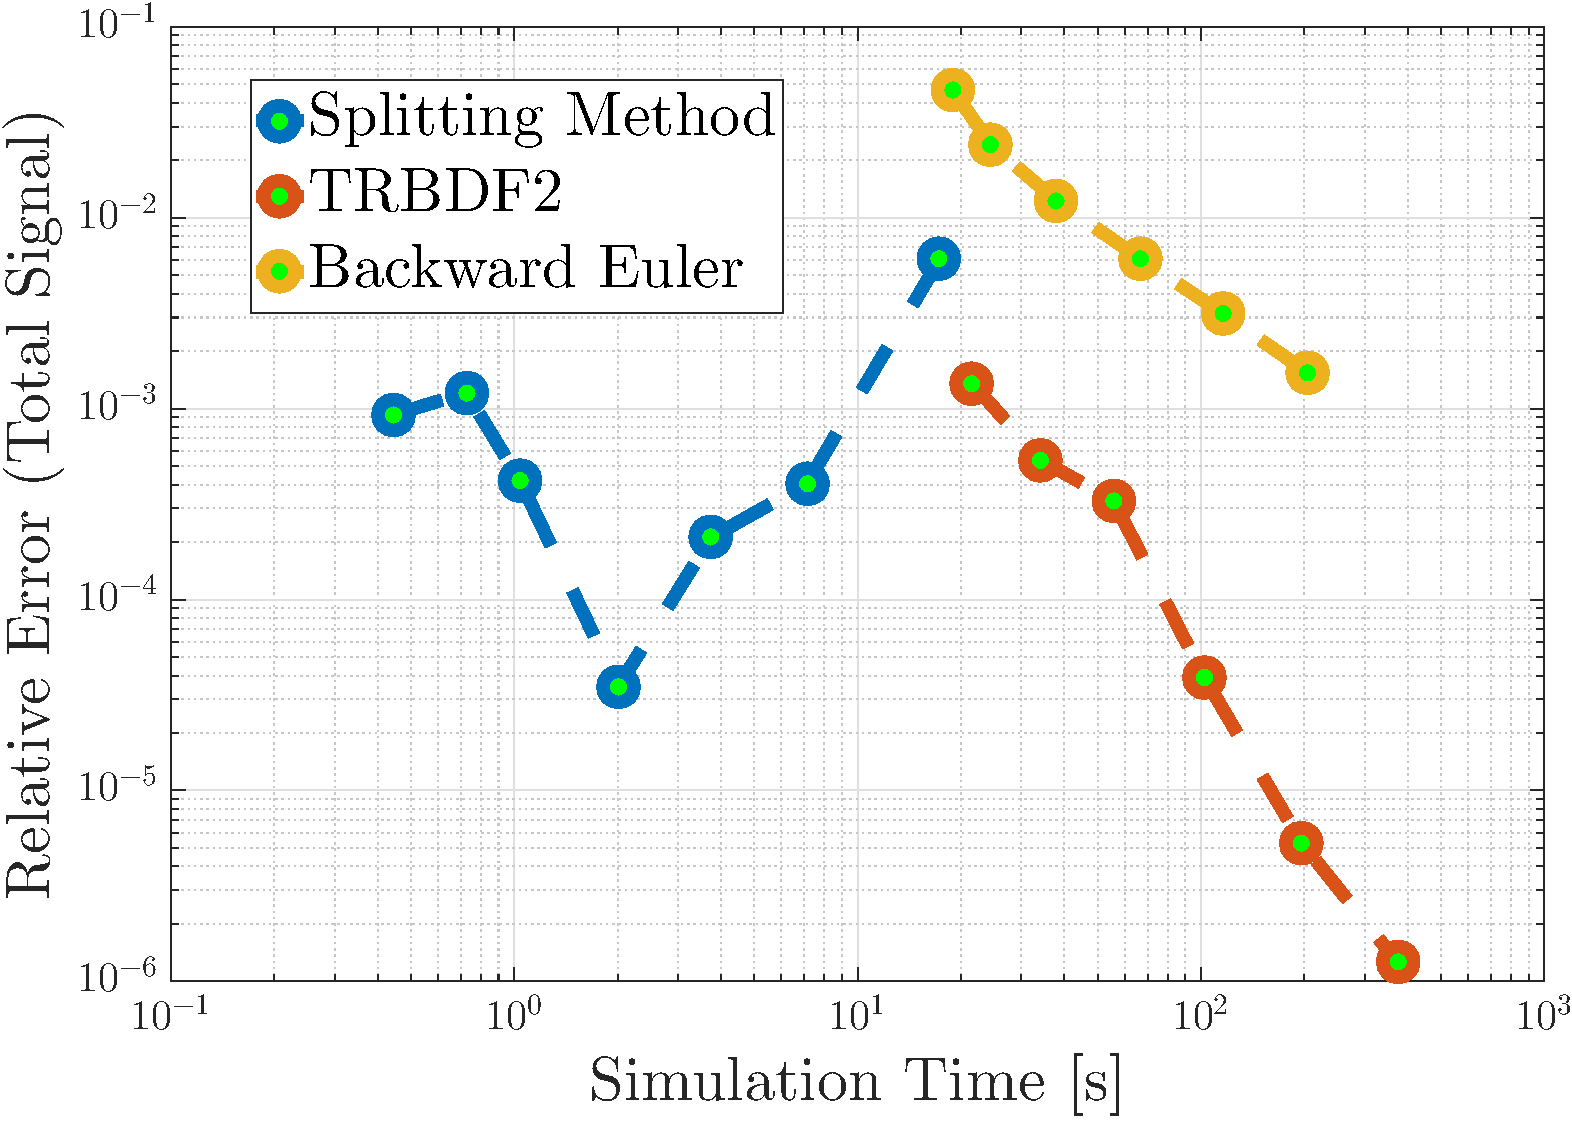
\includegraphics[width=0.9\linewidth]{figures/error_curves}
\end{frame}

\section{Conclusion}
\begin{frame}
\frametitle{Conclusion}
\Large
\begin{enumerate}
    \item Splitting methods:
    \begin{enumerate}
        \large
        \item[$+$] Fast
        \item[$-$] Resolution limitations
        \item[$\pm$] Periodic boundary conditions
    \end{enumerate}
    \pause
    \vspace{0.5cm}
    \item Finite element methods:
    \begin{enumerate}
        \large
        \item[$-$] Slow
        \item[$+$] Flexible boundary conditions
        \item[$+$] Adaptivity?
    \end{enumerate}
\end{enumerate}
\end{frame}

%\section{Acknowledgements}
%\begin{frame}
%\frametitle{Acknowledgements}
%\centering
%\vspace{-2.0cm}
%\huge Thank you
%\begin{textblock*}{3cm}(1.3cm,1cm)
%    
\includegraphics[height=3cm]{figures/ubc-logo}
%\end{textblock*}
%\begin{textblock*}{3cm}(6.8cm,1cm)
%    
\includegraphics[height=3cm]{figures/UBC-MRI-logo}
%\end{textblock*}
%\end{frame}

\end{document}
